\section{Microcontroller}
Like all engineering projects, our group needed a computer to handle our needs. The Raspberry Pi 3 is a programmable microcontroller that is compatible with the MPU we've selected. Figure \ref{rasp} shows an image of the microcontroller. The features offered by the Raspberry Pi are exactly what our team needs to begin a prototype. Below one will find the features that attracted us the most \cite{pi}. \hfill\newline
\begin{itemize}
    \item Cortex-A53 (ARMv8) 64-bit SoC
    \item Clock Speed: 1.4GHz
    \item 2.4GHz and 5GHz IEEE 802.11.b/g/n/ac wireless LAN, Bluetooth 4.2, BLE
    \item Gigabit Ethernet over USB 2.0 (maximum throughput 300 Mbps)
    \item Full-size HDMI
    \item 4 USB 2.0 ports
    \item Micro SD port for loading your operating system and storing data
\end{itemize}

\begin{figure}[H]
\centering
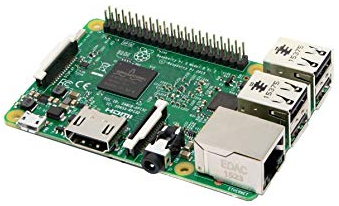
\includegraphics[width = 6.5cm,height = 4.5cm]{graphics/Raspberry.PNG}
\caption{Raspberry Pi}
\label{rasp}
\end{figure}

When it comes to the operating system, our team plans on using Ubuntu; an open-source Linux distribution. Our team comprises of two electrical engineers and five computer engineers, so navigating through the Linux terminal shouldn't be an issue. The team will also have the option to code in either C or Python. Because Python isn't a requirement in the computer engineering curriculum, this can be an opportunity for some of the team members to learn a new programming language.